\documentclass[aspectratio=169]{beamer}

\usepackage[utf8]{inputenc}
\usepackage{array}
\usepackage{booktabs}
\usepackage{bold-extra}
\usepackage{graphics}
\usepackage{hyperref}
\hypersetup{%
  colorlinks=true,
  linkcolor=blue,
  filecolor=blue,
  urlcolor=cyan,
}
\usepackage{listings}
\usepackage{multicol}
\usepackage[absolute,overlay]{textpos}
\usepackage{setspace}
\usepackage{verbatim}
\usepackage{fancyvrb} % for verbatim centering
\usepackage{tikz}

\usetheme{Warsaw}
\usecolortheme{beaver}
\definecolor{clOrange}{HTML}{E76600}
\definecolor{clAlmostWhite}{HTML}{FEFFD9}
\definecolor{clGreen}{HTML}{007F00}
\definecolor{clFlag}{HTML}{D33682}
\definecolor{clFlagOpt}{HTML}{CB4B16}
\definecolor{clRedFlag}{HTML}{DC322F}
\definecolor{clViolet}{HTML}{4c0070}
\definecolor{clGray}{HTML}{607060}

\definecolor{clCodeBlue}{rgb}{0.0, 0.18, 0.38}
\definecolor{clCodeGreen}{rgb}{0.0, 0.27, 0.15}
\definecolor{clCodeRed}{rgb}{0.63, 0.0, 0.0}


\setbeamertemplate{navigation symbols}{}
\setbeamercolor{title}{fg=black}
\setbeamercolor{author}{fg=clAlmostWhite}
\setbeamercolor{date}{fg=clAlmostWhite}
\setbeamerfont{author}{size=\huge}
\setbeamerfont{date}{size=\Large}

\newcommand{\greenemph}[1]{\textit{\textcolor{clGreen}{#1}}}
\newcommand{\cpp}[1]{\texttt{\textbf{\textcolor{clCodeBlue}{#1}}}}

\newcommand\fontV{\fontsize{5}{5}\selectfont}

\lstset{
  language=C++,
  basicstyle=\ttfamily,
  keywordstyle=\color{clCodeBlue}\ttfamily,
  stringstyle=\color{clCodeGreen}\ttfamily,
  commentstyle=\color{clCodeRed}\ttfamily,
  morecomment=[l][\color{magenta}]{\#}
}

\title[%
\texttt{\textcolor{clGray}{C++ Friends} %
\textcolor{clCodeBlue}{\#20}\textcolor{clGray}{~::~}\textcolor{clCodeBlue}{EfficiencyOfContainers}}%
]{%
Efficiency of C++ containers%
}
\author{gralin.ski}
\date{May 2022}

\begin{document}

{\usebackgroundtemplate{%
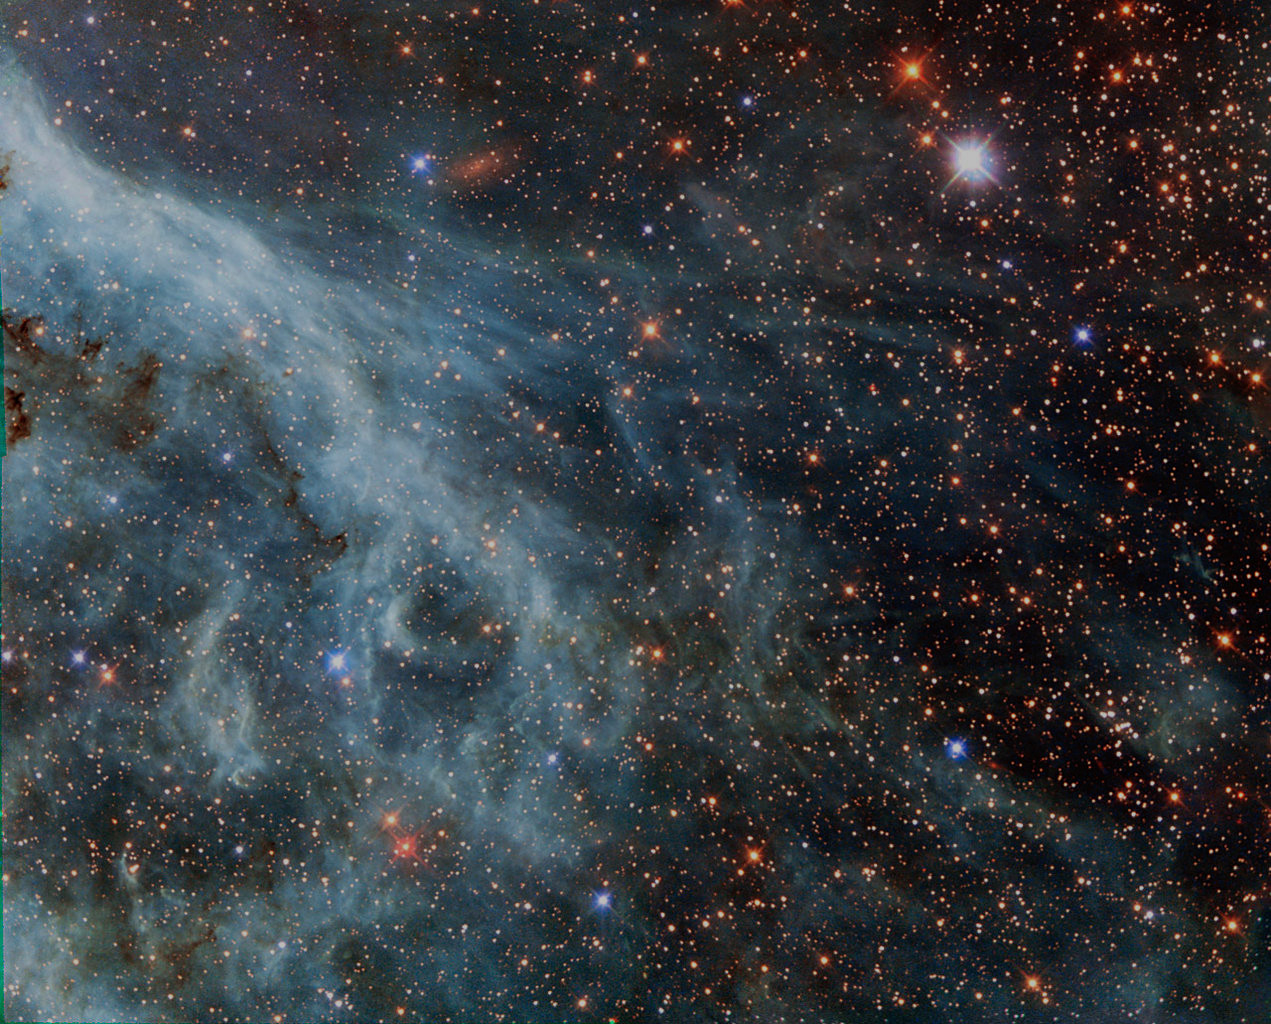
\includegraphics[width=\paperwidth,height=\paperheight]{../../common/bg_galaxy.jpg}}
\begin{frame}
\titlepage{}
\end{frame}
}

\begin{frame}
\frametitle{A quick reminder}
You are welcome to:
\begin{itemize}
  \item{interrupt me}
  \item{ask questions immediately}
\end{itemize}
\end{frame}

\begin{frame}[fragile]
\frametitle{cv-type qualifiers}
\href{https://en.cppreference.com/w/cpp/language/cv}{en.cppreference.com/w/cpp/language/cv}
\vspace{6pt}
  \begin{itemize}
    \item<2->{\cpp{const}}
    \begin{itemize}
      \item{defines that the type is \textit{constant} \hspace{2em} \uncover<5->{\textcolor{clGreen}{$\leftarrow{}$ (non-mutable)}}}
      \begin{lstlisting}
        const auto x = 13;
      \end{lstlisting}
    \end{itemize}

    \vspace{3pt}
    \item<3->{\cpp{(no qualifier)}}
    \begin{itemize}
      \item{the type is* a standard \textit{variable} \hspace{2.4em} \uncover<5->{\textcolor{clOrange}{$\leftarrow{}$ (mutable)}}}
      \begin{lstlisting}
        auto x = 13;
      \end{lstlisting}
    \end{itemize}

    \vspace{3pt}
    \item<4->{\cpp{volatile}}
    \begin{itemize}
      \item{the type is \textit{volatile} \hspace{7.8em} \uncover<5->{\textcolor{clRedFlag}{$\leftarrow{}$ (extremely mutable)}}}
      \begin{lstlisting}
        volatile auto x = 13;
      \end{lstlisting}
    \end{itemize}
  \end{itemize}
\end{frame}

\begin{frame}
\frametitle{Key takeaways}
{\centering
\begin{itemize}
  \item{Takeaway 1}
  \item{Takeaway 2}
\end{itemize}

\vspace{2ex}
\begin{center}{\Large Thank you!}\end{center}
}
\end{frame}

\end{document}
